%------------------------------------------------------------
% Description : Calculus in \R^n space
% Author      : taxus-d <iliya.t@mail.ru>
% Created at  : ??? 
%------------------------------------------------------------
\documentclass[12pt,timbord]{../../../notes}
\usepackage{silence}
\WarningFilter{latex}{Reference}
\WarningFilter{latex}{Citation}
\graphicspath{{../../img/}}

\begin{document}

\paragraph{Оценка приращения дифференцируемого отображения}
\label{par:diffspace::diffestim}

\begin{prop}\label{prop:diffspace::diffestim::lagrfail}
  Пусть $f\colon \R^n \to \R^m$, $m \geqslant 2$. Тогда формула Лагранжа
  \[
    f(b) - f(a) = f'(c)(b - a)
  \]
  не работает.
\end{prop}
\begin{exmp*}\label{exmp:diffspace::diffestim::lagrfail}
  Пусть 
  \[
    f(t) := (\cos t, \sin t),\; b - a = 2\pi
  \]
\end{exmp*}

\begin{thrm}[об оценке приращения отображения]\label{thrm:diffspace::diffestim::diffestim}
  Пусть $f\colon G \subset \R^n \to \R^m$, $G$~--- выпуклое, $f$~--- дифференцируема, 
  \[ 
    \forall\, x \in G \;\: \| f'(x) \| \leqslant M 
  \]
  Тогда $\forall\, a,b \in G \;\: \|f(b) - f(a)\| \leqslant M \| b-a \|$
\end{thrm}

\begin{ittproof}
  <<Окружим>>  исходную функцию:
  \[
    F = \psi \circ f \circ \varphi
  \]
  где \note{Вот тут как раз нужна выпуклость, иначе отрезок $[a;b]$ может и не лежать в $G$}
  \begin{align*}
    \varphi&: \R \to \R^n & \varphi(t) &:= t(b-a) + a, & t&\in [0,1] \\
    \psi&: \R^m \to \R & \psi(y) &:= \langle y, \ell \rangle, & \ell &= f(b)-f(a) 
  \end{align*}
  
  Заметим, что $F$~--- обычная вещественнозначная функция. Так что для неё работает формула
  Лагранжа:
  \[
    \exists\, c \in [0,1] \colon F(1)-F(0) = F'(c)(1-0) = F'(c)
  \]
  Тогда из свойств нормы (по ходу дела обозначим $\varphi(c)$ за $x$):
  \[
    \|F'(c)\| = \|\psi'(f(x)) \cdot f'(x) \cdot \varphi'(c)\| \leqslant 
    \|\psi'(f(x)) \| \cdot \| f'(x) \| \cdot \| \varphi'(c)\|
  \]
  Здесь тонкость в обозначениях. Производные~--- вроде матрицы, поэтому их нормы~--- что-то
  странное на первый взгляд. На самом деле смысл немного иной. 
  \[
    \mathrm d L(x, h) = f'(x) \cdot h
  \]
  Таким образом, дифференциал~--- неплохое линейное отображение. А под <<нормой производной>>
  имеется в виду норма соответствующего линейного отображения.

  Теперь давайте что-нибудь скажем про эти нормы. 

  \begin{enumerate}
    \item $\varphi'(t) = (b-a) \Rightarrow \| \varphi'(c) \| = \| b - a\|$
    \item $\psi(y) = \langle y, l \rangle$, $\| \psi\| = \|\ell\|$      
  \end{enumerate}
  Так что 
  \[
    \| F'(c)\| \leqslant M \cdot \| \ell \| \cdot \|b-a\|
  \]
  С другой стороны:
  \[
    F(1) - F(0) = \psi(f(b)) - \psi(f(a)) = \langle f(b), \ell \rangle - \langle f(a), \ell \rangle
    = \langle \ell, \ell \rangle  = \|\ell \|^2
  \]
  В итоге, совмещая оба выражения, приходим к утверждению теоремы.
\end{ittproof}

\paragraph{Частные производные высших порядков}
\label{par:diffspace::highpartial}

\begin{defn}\label{defn:diffspace::highpartial}
  Пусть $f \colon G \subset \R^n \to \R$, $\forall\, x\in G \;\: 
  \exists\, \partial^k_{i_1, \dotsc, i_{k}} f(x)$. Тогда
  \[
    \partial_{i_1, \dotsc, i_{k+1}}^{k+1} f(x) := \partial_{i_{k+1}}(\partial^k_{i_1, \dotsc, i_{k}} f) (x)
  \]
\end{defn}
\begin{rem}\label{rem:diffspace::highpartial::smooth}
  $C^p(G)$~--- класс функций, определённых в $G$ с непрерывной производной до $p$-го порядка
  включительно.
  Функции из $C^1$ ещё называются гладкими.
\end{rem}
  
\begin{thrm}[Зависимость производных $p$-го порядка от перестановки переменных]
  \label{thrm:diffspace::highpartial::permut}
  Пусть \mbox{$f \in C^p(G)$}, $x\in G$. При этом
  \[
    \begin{split}
      i &= \{ i_1, \dotsc, i_p \mid i_k \in \{1, \dotsc, n\}\} \\
      j &= \{ j_1, \dotsc, j_p \mid j_k \in \{1, \dotsc, n\}\} \\
      j &= \pi(i)
    \end{split}
  \]
  Тогда 
  $\partial_i^{\,p} f(x) = \partial_j^{\,p} f(x)$
\end{thrm}
\begin{ittproof}
  Сначала докажем всё для $p=2$, $n=2$, т.~е.
  \[
    \frac{\partial^2 f }{\partial x\partial y} =  \frac{\partial^2 f }{\partial y\partial x} 
  \]
  Пусть $(x, y) \in G$, $(x_0+ \Delta x, y) \in G$, $(x, y + \Delta y) \in G$,
  $(x + \Delta x, y + \Delta y) \in G$
  Введём ещё 2 функции:
  \begin{align*}
    \varphi(t) &= f(t, y+ \Delta y) - f(t, y) \\
    \psi(t) &= f(x+ \Delta x, t) - f(x, t)
  \end{align*}
  Тогда $\varphi(x+ \Delta x) - \varphi(x) = \varphi'(c_1) \Delta x = W$, 
  $c_1 \in [x, x+ \Delta x]$. При этом 
  \[
    W = \varphi'(x) \Delta x 
    \Delta x \left(\pder f x (c_1, y+ \Delta y) - \pder f x (c_1, y)\right) =  
    \pdder f x y (c_1, c_2) \, \Delta x \Delta y, \; c_2 \in [y, y+ \Delta y]
  \] 
  Аналогично
  \[
    W = \pdder f y x (c_3, c_4) \Delta x \Delta y, \; c_4 \in [y, y+ \Delta y], 
    c_3 \in [x, x+ \Delta x]
  \]
  По непрерывности второй производной $f$ $(f \in C^2)$
  \begin{align*}
    \pdder f x y (c_1, c_2) \xrightarrow[\substack{\Delta x \to 0 \\ \Delta y \to 0}]{} 
    \pdder f x y (x, y) \\
    \pdder f y x(c_3, c_4) \xrightarrow[\substack{\Delta x \to 0 \\ \Delta y \to 0}]{} 
    \pdder f y x(x, y)
  \end{align*}
  По теореме о предельном переходе в равенствах $\ddot\smile$ смешанные производные равны.

  Теперь поймём, что делать в случае произвольных $p, n$. 

  Представим подстановку $\pi$ как произведение транспозиций соседних элементов. Будем дальше
  разбираться с такими транспозициями. 
  
  Пусть $\tau_k = (j,j+1)$. Сначала посчитаем производные по $x_1, \dotsc, x_{j-1} = i'$.
  А теперь обозначим $\widetilde{f} = \partial_{i'} f$. По доказанному утверждению для двух
  переменных, $\partial_{j,j+1} \widetilde{f} = \partial_{j+1,j} \widetilde{f} $. А теперь
  продифференцируем это равенство по оставшимся переменным.

  Таким образом, для произвольной транспозиции $\tau_k = (j, j+1)$ верно утверждение теоремы. 
  А значит, и для произвольной подстановки $\pi = \prod_k \tau_k$ теорема верна. 
\end{ittproof}
\begin{rem}\label{rem:diffspace::highpartial::permut}
  Тут важно, что $f\in C^p(G)$. Одной точки бы не хватило, мы
  ведь рассматриваем маленький параллелепипед в $U(x)$ и используем одномерную теорему
  Лагранжа внутри него. А для неё нужна дифференцируемость на интервале.
\end{rem}

\paragraph{Обобщение бинома}
\label{par:diffspace::genbinom}
<<Обычный>> бином Ньютона:
\[
  (a+b)^n  = \sum_{k=0}^n C_n^k a^k b^{n-k}
\]
Его нетрудно обобщить до полинома Ньютона
\[
  (a_1 + \dotsb + a_n)^p = \sum_{i_1=1}^n \sum_{i_2=1}^n \dotsi \sum_{i_p=1}^n a_{i_1} \dotsm a_{i_p}
  = \sum_{{\substack{\mathclap{\alpha_i \in \{0, \dotsc, p\}}\\ \sum \alpha_i = 1}}} 
  a_1^{\alpha_1} \dotsm a_n^{\alpha_n} \cdot C_{\alpha_1, \dotsc, \alpha_n} 
\]
Введём обозначения:
\begin{itemize}
  \item $a = (a_1, \dotsc, a_n)$
  \item $\alpha = (\alpha_1, \dotsc, \alpha_n)$~--- мультииндекс, по сути вектор индексов, для
    которого вводится своя куча обозначений, дабы упростить жизнь
    \begin{enumerate}
      \item $\alpha + \beta = (\alpha_i + \beta_i)_{i=1}^n$
      \item $|\alpha| = \sum_{i=1}^n\alpha_i$
      \item $\alpha! = \prod_{i=1}^n\alpha_i!$
    \end{enumerate}
  \item $a^\alpha = \prod_{i=1}^n a_i^{\alpha_i}$
  \item $\partial_\alpha = \partial^n_{\alpha_1, \dotsc, \alpha_n} = \dfrac{\partial^n f}{\partial
    x_{\alpha_1} \dotso \partial x_{\alpha_n}}$
  \item $C_\alpha = C_{\alpha_1, \dotsc, \alpha_n}$
\end{itemize}

\begin{prop}\label{prop:diffspace::genbinom::factors}
  $\displaystyle C_\alpha = \frac{p!}{\alpha!}$
\end{prop}
\begin{itlproof}
  Ну, это просто число перестановок с повторениями. Нужно взять по множителю из $p$ скобок,
  причём перестановки одинаковых множителей входят в одно слагаемое. В итоге нужно делить общее
  число перестановок на число перестановок одинаковых множителей. А дальше можно сказать, что
  в каждое слагаемое входит каждый множитель, просто некоторые в нулевой степени.
\end{itlproof}

\paragraph{<<Многомерный>> дифференциал высоких порядков. Формула Тейлора для функций многих
переменных}
\label{par:diffspace::highdifftaylor}

\begin{defn}\label{defn:diffspace::highdiff}
  Пусть $f \colon G \subset \R^n \to \R$, $f\in C^p(G)$. Тогда
  \[  
    \del^p f(x) := \sum_{1 \leqslant i_1 \leqslant \dotsb \leqslant i_p \leqslant n}
    \frac{\partial^p f}{\partial x_{i_1} \dotso \partial x_{i_p}} \, \del x_{i_1} \dotsm \del x_{i_p}
  \]
  Или ещё можно вот так записать
  \[
    \left(\sum_i \del x_i\, \partial_i \right)^p f(x)
  \]
\end{defn}

\begin{stat}\label{stat:diffspace::highdiff::binom}
  Если частные производные можно переставлять, то
  \[
    \del^p f(x) = \sum_{\substack{0 \leqslant \alpha_i \leqslant p \\ |\alpha_i| = p}} 
    \frac{p!}{\alpha!} \, \partial_\alpha f(x) \,\del x ^ \alpha
  \]
\end{stat}

\begin{thrm}\label{thrm:diffspace::taylor}
  Пусть $f \in C^{p+1}(G), G\in \R^n$,$G$~--выпуклая, $a\in G$. 
  Пусть также $h\in \R^n \colon a+h \in G$.
  Тогда 
  \[
    f(a+h) = \sum_{k=0}^p \frac{1}{k!} \, \del^k f(a,h) + R_p(h)
  \]
  Остаток $R_p(h)$ можно представить несколькими способами:
  \begin{enumerate}
    \item В форме Пеано: $R_p(h) = o(\|h\|^p)$
    \item В форме Лагранжа: $R_p(h) = \dfrac{1}{(p+1)!}\, \del^{p+1} f(a + \theta h, h)$, 
      $\theta \in (0,1)$
  \end{enumerate}
\end{thrm}
\begin{ittproof}
  Рассмотрим $\varphi(t) = a + t h$, $t\in [0,1]$, $F(t) = f(\varphi(t))$, $F\colon [0,1]\to \R$.
  По одномерной теореме Тейлора 
  \[
    F(1) = F(0)+ 1\cdot F'(0) + \frac{1}{2!} F''(0) 1^2 + \dotsb + \frac{1}{p^2} F^{(p)}(0) \cdot
    1^p + R_p
  \]
  Докажем, что $F^{(k)}(0) = \del ^k f(a,h)$.
  Проще всего по индукции, давайте ещё такое нестандартное обозначение введём: 
  $(k) = (1, \dotsc, k)$, и будем понимать под $i_{(k)}$ вектор индексов, а под 
  $h_{i{(k)}}$~--- произведение соответствующих $h$.
  \begin{description}
    \item[база:] $F(0) = f(a)$
    \item[переход:] Пусть $F^{(k-1)}(t) = \dsum_{1 \leqslant i_1, \dotsc, i_{k-1} \leqslant n } \,
      \partial_{i_{(k-1)}} f(a + th) \, h_{i_{(k-1)}}$. При дифференцировании по t всякие
      $h_{i_j}$ в каждом слагаемом вынесутся за знак производной, а частная производная от $f$
      даст $\sum_{i_k} \partial_{i_{(k)}} f(a+ht) h_{i_k}$. Если скомпоновать все суммы и
      подставить $t=0$, как раз получается $d^k f(a,h)$
  \end{description}

  Теперь разберёмся с остатком
  \[
    R_p = \frac{1}{(p+1)!}F^{(p+1)}(\theta)\cdot1^{p+1}=\frac{1}{(p+1)!}\del^{(p+1)}f(a+h\,\theta, h) 
  \]
  Поскольку $\forall\, i\;\: |h_i| \leqslant \|h\|$
  \[
    d^{(p+1)} f(a+\theta\, h , h) = O(\|h\|^{p+1}) = o(\|h\|^p)
  \]
  Следовательно, $R_p = o(\|h\|^p)$
\end{ittproof}

\paragraph{Понятие экстремума, необходимое условие}
\label{par:diffspace::extrema::ness}

\begin{defn}\label{defn:diffspace::extrema}
  Пусть $f\colon G \subset \R^n \to \R$, $a\in G$. Тогда говорят, что $f$ имеет в $a$ максимум (нестрогий), если
  \[
    \exists\, U(a) \colon \forall\, x \in U \;\: f(x) \leqslant f(a)
  \]
  Когда неравенство строгое, а окрестность проколотая, то максимум~--- строгий
  Для минимума нужно $\geqslant$.
\end{defn}

\begin{thrm}[Необходимое условие экстремума]\label{thrm:diffspace::extrema::ness}
  Пусть $a$ внутренняя точка $G \subset \R^n$, $f\in C^1(a)$. Тогда если $f$ имеет в $a$ экстремум, то
  \[
    \del f(a) = 0 \Leftrightarrow \forall\,i \;\: \partial_i f(a) = 0
  \]
\end{thrm}
\begin{ittproof}
  Рассмотрим $\varphi_i(t) = f(a_1, \dotsc, a_{i-1}, t, a_{i+1}, \dotsc, a_n)$. Тогда у такой
  функции есть экстремум в $a_i$. А тогда, из одномерной теоремы Ферма $d \varphi_i(t) = 0$. А
  значит $\partial_i f =0$
\end{ittproof}


\paragraph{Про квадратичные формы }
\label{par:diffspace::quadforms}
\begin{defn}\label{defn:diffspace::quadforms::bilin}\note{тут изложение больше по \cite{gelfand}} 
  Функция $A\colon V \times V \to \R$, где $V$~--- векторное пространство,
  называется \emph{билинейной формой}, если она линейна по обеим своим аргументам.
\end{defn}

\begin{defn}\label{defn:diffspace::quadforms::bilinsym}
  Билинейная форма $A$ называется \emph{симметрической}, если $\forall\, x, y \;\: A(x,y)=A(y,x)$.
\end{defn}

\begin{defn}\label{defn:diffspace::quadforms::bilinmtx}
  Пусть $A$~--- билинейная форма, $e_1, \dotsc, e_n$~--- базис в векторном пространстве.
  Тогда \[
    A (x,y) = \sum_{i,j=1}^n A(e_i, e_j) x^i y^j
  \]
  и матрица $A$, элементы которой $a_{ij} =  A(e_i, e_j)$ называется матрицой билинейной формы.
\end{defn}

\begin{defn}\label{defn:diffspace::quadforms::quad}
  Пусть $A$~--- симметрическая билинейная форма. Тогда $A(x)=A(x,x)$~--- \emph{квадратичная форма}.
  При этом $A(x,y)$ называется \emph{полярной формой} по отношению к $A(x)$.
\end{defn}

\begin{defn}\label{defn:diffspace::quadforms::quadmtx}
  Матрица квадратичной формы~--- матрица соответствующей полярной формы.
\end{defn}

\begin{defn}[<<Определённость>> формы]\label{defn:diffspace::quadforms::sign}
  Если что-то верно, то про форму $A(x,y)$ говорят:
  \begin{itemize}
    \item $\forall\, x,y \neq 0 \;\: A(x,y) > 0$~--- положительно определена
    \item $\forall\, x,y \neq 0 \;\: A(x,y) < 0$~--- отрицательно определена
    \item $\forall\, x,y \neq 0 \;\: A(x,y) \geqslant 0$~--- полуопределена в положительном смысле
    \item $\forall\, x,y \neq 0 \;\: A(x,y) \leqslant 0$~--- полуопределена в отрицательном смысле
  \end{itemize}
\end{defn}

\begin{exmp*}
  Скалярное произведение~--- положительно определённая билинейная форма.
\end{exmp*}

\begin{thrm}\label{thrm:diffspace::quadforms::orthodiag}
  Пусть в некотором базисе $f_1, \dotsc, f_n$ квадратичная форма $A$ имеет матрицу $(a_{ij})$.
  Пусть к тому же все <<северо-западные>> миноры $\Delta_i$ отличны от нуля. 
  Тогда существует базис $e_1, \dotsc,e_n$, в котором матрица $A$ имеет вид
  \[
    \begin{pmatrix}
      \frac{1}{\Delta_1} & & &\\
      & \frac{\Delta_1}{\Delta_2} & & \\
      & & \ddots & \\
      & &  & \frac{\Delta_{n-1}}{\Delta_n}
    \end{pmatrix}
  \]
\end{thrm}
\begin{ittproof}
  По сути, нам нужно построить ортогональный базис, только вместо скалярного произведения
  используется билинейная форма $A$(причём не обязательно положительно определённая).
  За подробностями см.~\cite{gelfand}.
\end{ittproof}

\begin{thrm}[Правило Сильвестра]\label{thrm:diffspace::quadforms::silv}
  Квадратичная форма положительно определена, если все миноры из
  теоремы~\ref{thrm:diffspace::quadforms::orthodiag} положительны, и отрицательно определена, если
  их знаки чередуются, начиная с <<->>.
\end{thrm}
\begin{ittproof}
  Следствие предыдущей теоремы. Определённость формы не зависит от выбора базиса.
\end{ittproof}

\paragraph{Достаточное условие экстремума}
\label{par:diffspace::extrema::suff}

\begin{thrm}[Достаточное условие экстремума]\label{thrm:diffspace::extrema::suff}
  Пусть $a\in G \subset \R^n$, $a$~--- внутренняя точка, $f\in C^2(a)$.
  \begin{enumerate}
    \item $\del f(a) = 0$, $\del^2 f(a,h) > 0 \Rightarrow$ $f$ имеет в $a$ $\min$
    \item $\del f(a) = 0$, $\del^2 f(a,h) < 0 \Rightarrow$ $f$ имеет в $a$ $\max$
    \item $\del f(a) = 0$, $\del^2 f(a,h) \lessgtr 0 \Rightarrow$ ничего нет
    \item $\del f(a) = 0$, $\del^2 f(a,h) \leqslant 0 \Rightarrow$ $f$ не имеет в $a$ $\min$
    \item $\del f(a) = 0$, $\del^2 f(a,h) \geqslant 0 \Rightarrow$ $f$ не имеет в $a$ $\max$
  \end{enumerate}
\end{thrm}
\begin{ittproof}
  Поскольку $\del f(a) = 0$,  $\Delta f(a) = \frac 1 2 (\del^2 f(a) + \alpha)$, 
  где $\alpha = o(\|h\|)$. Для упрощения жизни примем $t=\frac{h}{\|h\|}$. Тогда приращение
  функции можно переписать в виде
  \[
    \Delta f  = \|h\|^2 \left( \frac{1}{2} \sum b_{ij} t_i t_j + \frac\alpha{\|h\|^2} \right)
  \]
  Поскольку $\frac{\alpha}{\|h\|^2} \to 0$, существует $\overset{\circ}{U}_\varepsilon (a)$ в которой 
  знак приращения определяется лишь первым слагаемым. Нетрудно заметитить, что все значения $t$
  лежат на единичной сфере, которая компакт. Причём значения $t$ покрывают всю сферу, ведь
  направление $h$ можно выбирать в окрестности $a$ произвольно. Так что можно просто сделать
  второе слагаемое меньшим минимума квадратичной формы на единичной сфере.

  Таким способом можно расправиться с пунктами 1--2. 

  Для пункта 3 отыщем $h_1 \colon \del^2(a, h_1) > 0$, $h_2 \colon \del^2(a, h_1) < 0$. Заметим,
  что если $A$~--- квадратичная форма, 
  то $A(h)>0$ $\Rightarrow$ $ \forall\,s \;\: A(sh)=s^2\,A(h) > 0 $. По сути, мы считаем значение
  формы вдоль прямой, проходящей через $a$. 
  Если, как и выше, записать приращение в виде
  \[
    \Delta f  = s^2 \left(\frac 1 2 \,\del^2 (a, h_{1|2}) + \frac\alpha{s^2}\right)
  \]
  то видно, что можно получить в окрестности $\pneigh U (a) $ всё, что угодно, просто $s\to 0$.

  4--5 легко доказываются от противного.
\end{ittproof}
%% не нужно нафиг, есть более общая теорема дальше. Тут костыли какие-то
% \paragraph*{Понятие о неявной функции}
% \label{par:diffspace::implicit2}

% \begin{defn}\label{defn:diffspace::implicit2}
%   Пусть $F\colon G \subset \R^2 \to \R$. Рассмотрим уравнение
%   \begin{equation}
%     \label{eq:diffspace::implicit2::base}
%     F(x, y) = 0
%   \end{equation}

%   Пусть $a =(x_0, y_0)$ удовлетворяет \eqref{eq:diffspace::implicit2::base}, 
%   а $U$~--- окрестность $a \colon$ $U = U_x \times U_y$.
%   Тогда будем говорить, что уравнение \eqref{eq:diffspace::implicit2::base} определяет неявную 
%   функцию $f$ в $U$, если
%   \[
%     \forall\, x\in P \; \exists!\, y\in Q \colon F(x,y) = 0 \hspace{1.5em} (y = f(x))
%   \]
% \end{defn}

% \begin{thrm}[О неявной функции]\label{thrm:diffspace::implicit2}
%   Пусть $F\colon G\subset \R^2 \to \R$, $F\in C^1(x_0,y_0)$, а $a=(x_0, y_0) \colon$
%   \begin{enumerate}
%     \item $F(x_0, y_0) = 0$
%     \item $F_y'(x_0, y_0) \neq 0$
%   \end{enumerate}
%   Тогда 
%   $\exists\, P(x_0), Q(y_0) \colon $ в $U = P\times Q$ уравнение \eqref{eq:diffspace::implicit2::base} 
%   задаёт неявную функцию $f\colon P\to Q$. При этом
%   \[
%     f\in C^1 \land f'(x) = - \frac{F_x'(x,y)}{F_y'(x,y)}
%   \]
% \end{thrm}
% \begin{ittproof}
%   \begin{enumerate}
%     \item (Доказательство существования) \\
%       Рассмотрим $\varphi(y) = F(x_0, y)$. Пусть НУО $F_y'(x_0, y_0) > 0$.
%       Тогда 
%       \[
%         \exists\, U_\varepsilon(x_0, y_0) \colon \forall\, x, y \in U \;\: F_y'(x, y) > 0
%       \]
%       Обозначим соответствующие проекции $U$ (шар) на координатные оси за $U_x, U_y$
%       Получается, что $\varphi \uparrow U_y = (y_0 - \varepsilon; y_0 + \varepsilon)$.
%       Тогда 
%       \[
%         \begin{split}
%           \exists\, V_1(x_0) &\colon \forall\, x\in V_1 F(x, y+\varepsilon) > 0 \\
%           \exists\, V_2(x_0) &\colon \forall\, x\in V_2 F(x, y-\varepsilon) < 0 \\
%                            P &= V_1 \cap V_2
%         \end{split}
%       \]
%       Тогда из теоремы Больцано-Коши и монотонности $\varphi$
%       \[
%         \forall\, x \in P \; \exists!\, y\in Q=U_y \colon F(x, y) = 0
%       \]
%       В итоге получилось определение неявной функции.
%     \item Непрерывность в $(x_0, y_0)$ вроде очевидна, мы же каждому $x$ из $\tilde P \subset P$
%       сопоставили 1 $y$ из $\tilde Q \in Q$. 
%       Принадлежность классу $C$ можно установить проведя аналогичные рассуждения
%       для $x\in P(x_0)$
%     \item С гладкостью что-то странное. Можно наверное сделать как в Зориче (через приращения и
%     теорему о среднем)
%     \item $F(x, f(x)) \equiv 0 \Rightarrow F_x'\cdot 1 + F_2'f'(x) = 0$
%   \end{enumerate}
% \end{ittproof}

\paragraph{Полнота пространства \texorpdfstring{$\R^n$}{}}
\label{par:diffspace::banach}

\begin{defn}\label{defn:diffspace::banach::cauchyseq}
  Последовательность $(x_n)$ называется фундаментальной (последовательностью Коши),
  если 
  \[
    \forall\, \varepsilon > 0 \;\: \exists\, N\colon \forall\,m,n>N \;\: \rho(x_n - x_m) < \varepsilon 
  \]
\end{defn}

\begin{defn}\label{defn:diffspace::banach::comtmetspc}
  Метрическое пространство $(X,\rho)$~--- полное, если всякая фундаментальная последовательность
  в нём  сходится
\end{defn}

\begin{exmp*}
  $\R \setminus 0$~--- не полное метрическое пространство, $x_n = \lfrac{1}{n}$ тому пример.
\end{exmp*}

\begin{rem}\label{rem:diffspace::banach::clos}
  Если $(X, \rho)$~--- полно, то $X$ вообще-то замкнуто. Хорошо видно на примере выше.
\end{rem}
\begin{rem}\label{rem:diffspace::banach::closubset}
  Если $(X, \rho)$~--- полно, $Y \subset X$~--- замкнуто. Тогда и $Y$~--- полно.
\end{rem}

\begin{stat}\label{stat:diffspace::banach::comtRn}
  $\R^n$~--- полное метрическое пространство.
\end{stat}
\begin{itlproof}
  $\sphericalangle$ произвольный $\varepsilon > 0$. Тогда 
  \[
    \rho(x_n - x_m) < \varepsilon 
    \Rightarrow \forall\, i \;\: \rho(x_m^i e_i - x_n^i e_i) < \varepsilon
    \Rightarrow \forall\, i \;\: |x_m^i - x_n^i| < \varepsilon
  \]
  Таким образом $(x_n^i)\in \R$~--- фундаментальная. 
  А в $\R$ по теореме из первого семестра фундаментальные последовательности сходятся.
  Тогда $\forall\, x_n^i \to a^i$. Значит и $x_n \to a$. 
\end{itlproof}

Кусок дальше не шибко нужен

\begin{itaux}
  Давайте введём метрику на пространстве непрерывных функций
  \begin{defn}\label{defn:diffspace::banach::cont}
    Пусть $f, g, h \in C\bigl([a;b]\bigr)$. Тогда 
    \[
      \rho(f,g) := \sup_{x\in [a;b]} |f(x) - g(x)| = \|f - g\|
    \]
  \end{defn}
  Здесь супремум можно заменить на максимум по теореме Вейерштрасса.

  Докажем что это правда расстояние:
  \begin{itemize}
    \item $\rho(f,g) =\rho (g,f)$~--- очевидно
    \item $\rho(f,g) \geqslant 0$~--- тоже очевидно
    \item $\rho(f,g) = \rho(f,h) + \rho(h,g) $~--- не так очевидно
      \[
        \begin{split}
          \max_{x\in [a;b]}|f(x)-g(x)| = |f(x_0) - g(x_0) | 
          &\leqslant |f(x_0) - h(x_0)| + |h(x_0)-g(x_0)|\\
          &\leqslant \max_{x\in [a;b]}|f(x) - h(x)| + \max_{x\in [a;b]}|h(x)-g(x)|
          = \rho(f,h) + \rho(h,g)
        \end{split}
      \]
  \end{itemize}

  \begin{prop}\label{prop:diffspace::banach::contcomp}
    Пространство $C\bigl([a;b]\bigr)$ с указанной выше метрикой полно.
  \end{prop}
  \begin{itlproof}
    Поточечная сходимость очевидна из полноты $\R$. А равномерную можно получить, устремив $m$ к
    $\infty$, зафиксировав $n$. А из равномерной сходимости следует непрерывность предельной
    функции.
  \end{itlproof}
  \begin{rem*}
    Если взять в качестве метрики $\int_a^b |f-g|$, то полнота поломается. Пополнение будет
    пространством суммируемых функций.
  \end{rem*}
\end{itaux}
\paragraph{Теорема о сжимающем отображении}
\label{par:diffspace::contrmap}

\begin{defn}\label{defn:diffspace::contrmap}
  Пусть $(X, \rho)$~--- метрическое пространство. Тогда отображение $T\colon X \to X$ называется
  сжимающим, если 
  \[
    \exists\, C \in (0,1) \colon \forall\, x',x'' \rho(T(x'), T(x'')) 
    \leqslant C\cdot \rho(x',x'')
  \]
\end{defn}

\begin{thrm}[Банах]\label{thrm:diffspace::contrmap::banach}
  Пусть $(X, \rho)$~--- полное метрическое пространство, а отображение $T\colon X \to X$~--- сжимающее.
  Тогда $\exists!\, x_* \in X \colon Tx_* = x_*$ (неподвижная точка).

  Ещё часто ссылаются на следующий факт, появляющийся в процессе доказательства:
  \[
    \forall\, x_0 \in X \; \exists\, \lim_{n\to \infty} T^n x_0 = x_*
  \]
\end{thrm}
\begin{ittproof}
  $\sphericalangle$ $x_n = T^n x_0$, где $x_0\in X$~--- произвольное. Докажем, что 
  \begin{enumerate}
    \item $x_n \to x_*$
    \item $T x_* = x_*$
    \item других таких $x_*$ нет.
  \end{enumerate}

  Поехали
  \begin{enumerate}
    \item $(x_n)$ сходится в себе, ведь $C\in (0,1)$.
      \[
        \rho(x_m, x_{m+p}) \leqslant \rho(x_m, x_{m+1}) + \dotsb + \rho(x_{m+p-1}, x_{m+p})
        \leqslant \rho(x_0, x_1) C^m (1 + \dotsb + C^{p-1})
          < \rho(x_0, x_1)\,\frac{C^m}{1-C} \xrightarrow[m\to \infty]{} 0
      \]
      раз пространство полное, $\exists\, \lim_{\infty} x_n$
    \item отображение $T$ непрерывно $ \Rightarrow $ $T x_n \to T x_*$. Но по теореме о
      подпоследовательности и единственности предела $T x_* = x_*$.
    \item Пусть $x_{**}$~--- другая неподвижная точка. Но тогда 
      % сгенереровано, нечитайте
      \[
        \rho \left( x_{\ast \ast} , x_{\ast} \right) = \rho \left( T x_{\ast
        \ast} ,T x_{\ast} \right) \leqslant C \rho \left( x_{\ast \ast} ,
        x_{\ast} \right) \Rightarrow \left( C - 1 \right) \rho \left( x_{\ast \ast}
        , x_{\ast} \right) \geqslant 0 \xRightarrow[C < 1]{} \rho \left( x_{\ast
        \ast} , x_{\ast} \right) = 0 
      \]
  \end{enumerate}

\end{ittproof}

\paragraph{Метод Ньютона}
\label{par:diffspace::newtfindroot}

Пусть $f\in C\bigl([a;b]\bigr)$, $f(a)\cdot f(b)$, $f(x_*) = 0$ , $f'(x_*) \neq 0$. 
Сам метод выглядит как-то так:

\noindent
Проводится касательная к графику в текущей точке, ищется её пересечение с осью $x$, 
оттуда восставляется перпендикуляр, пересечение которого с графиком~--- новая точка.
\[
  x - T x = \frac{f(x)}{f'(x)} \Leftrightarrow Tx = x - \frac{f(x)}{f'(x)}
\]

Докажем, что это вообще работает.
\begin{thrm}\label{thrm:diffspace::newtfindroot}
  Пусть $f\in C^2\left([a;b]\right)$, $x_* \in [a;b]$:
  \begin{enumerate}[a)]
    \item $f(x_*) = 0$
    \item $f'(x_*) \neq 0$
  \end{enumerate}
  Тогда $\exists\, U(x_*) \colon \forall\, x_0 \in U$, такая что $T^n x_0 \to x_*$ и
  $x_{n+1} - x_* = O\bigl((x_n -x_*)^2\bigr)$
\end{thrm}
\begin{ittproof}
  Сначала оценим $T'$.
  \[
    T'(x) = 1 - \frac{f'(x)^2 - f(x)f''(x)}{f'(x)^2} = \frac{f(x)f''(x)}{f'(x)^2} 
    \xrightarrow[n\to \infty]{(f\in C^2)} \frac{f(x_*)f''(x_*)}{f'(x_*^2)} 
    = 0
  \]
  Так что $\exists\, U(x_*) \colon c \in \overline{U} \Rightarrow |T'(c)| \leqslant \lfrac 1 2$.
  
  Теперь покажем, что $T(\overline{U}) \subset \overline{U}$. Из вышесказанного
  \begin{equation}
    |Tx - Tx_*| \leqslant \frac{1}{2} |x-x_*|
    \label{eq:diffspace::newtfindroot::contrnewt}
  \end{equation}
  Поскольку $Tx_* = x_* - 0 = x_*$, то \eqref{eq:diffspace::newtfindroot::contrnewt} равносильно
  \[
    | Tx - x_* | \leqslant \frac{1}{2} |x-x_*| 
  \]
  А это как раз то, что надо. 
  Значит $T$ как раз сжимающее отображение, и  по теореме \ref{thrm:diffspace::contrmap::banach} 
  такой $x_*\colon f(x_*) = 0$ единственный.

  Вторая часть тривиально получается из разложения $f$ в ряд Тейлора в окрестности $x_n$.
\end{ittproof}

\paragraph{Теорема об обратном отображении(формулировка)}
\label{par:diffspace::invmaphandwave}

Пусть $F: G\subset \R^n \to \R^m$~--- гладкое. Порассуждаем, когда может существовать $F^{-1}$.

Рассмотрим, например, линейное отображение.
\[
  y = F(x) = Ax \Leftrightarrow 
  \begin{cases}
    y_1 = a_{11} x_1 + \dotsb + a_{1n} x_n \\
    \hdotsfor{1}\\
    y_m = a_{m1} x_1 + \dotsb + a_{mn} x_n
  \end{cases}
\]

Понятно, что в таком случае задача поиска обратного отображения сводится к поиску обратной матрицы.
Тогда из линала ясно, что для того, чтобы у нас всё вышло, нужно
\[
  m = n \land \det A \neq 0 
\]

Теперь попытаемся обобщить на остальные функции. 

Пусть $a\in G$, $b = F(a)$
\[
  (?) \exists\, U(a), V(b) \,\colon \: F\colon U \leftrightarrow V
\]

\begin{figure}[h]
  \centering
  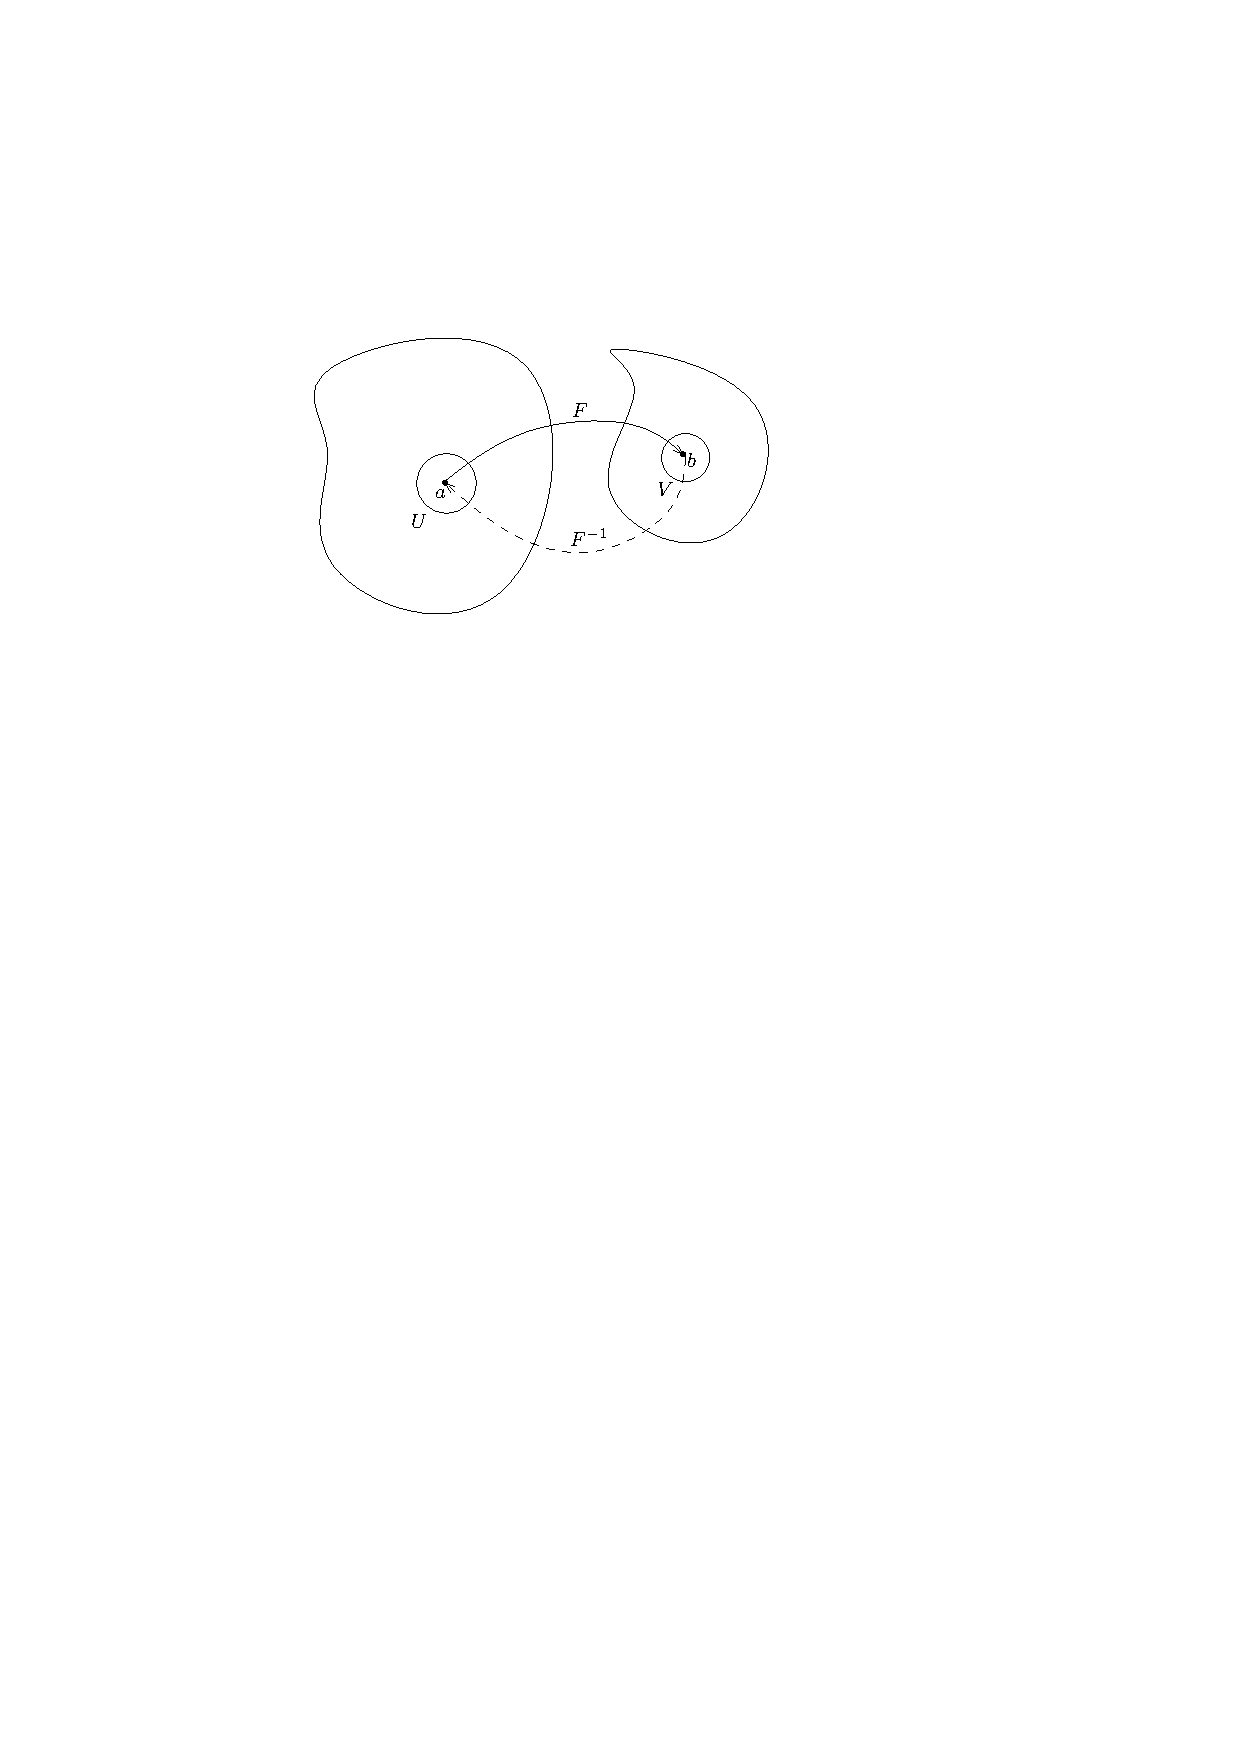
\includegraphics[width=0.6\linewidth]{inversemap}
\end{figure}

\begin{align}
  \Delta F &= F(x) - F(a) = y - b = \Delta y \label{eq:diffspace::invmaphandwave::delta}\\
  \Delta F &= F'(a) dx + o(dx) \\
  \del F(a) &= \del y(b) \label{eq:diffspace::invmaphandwave::diff}
\end{align}

Условие разрешимости \eqref{eq:diffspace::invmaphandwave::diff}~--- $\det\bigl(F'(a)\bigr) \neq 0$.
Утверждается, что у \eqref{eq:diffspace::invmaphandwave::delta} условие разрешимости такое же.

Соответственно, формулировка 
\begin{thrm}\label{thrm:diffspace::invmap}
  Пусть $F\colon G\subset \R^n \to \R^n$, $a\in G$, $b = F(a)$. Пусть ещё $F \diffin a$, 
  $\det(F'(a)) \neq 0$
  
  Тогда 
  \[
    \begin{split}
      & \exists\, U(a), V(b) \,\colon\; F \colon U \leftrightarrow V \\
      & \exists\, F^{-1} \colon V\to U, \; F^{-1} \in C^0
    \end{split}
  \]
\end{thrm}

\paragraph{Доказательство теоремы об обратимости}
\label{par:diffspace::invmapproof}

\begin{ittproof}[Теорема об обратимости отображения]
  Введём обозначения:
  \begin{align*}
    F'(a) &= \Gamma\\
    \Phi(x) &= x - \Gamma^{-1} (F(x) - y)
  \end{align*}
  Нетрудно заметить, что $x$~--- неподвижная точка $\Phi$ $\Leftrightarrow F(x)=y$ .
  Очень хотелось бы подогнать всё под теорему Банаха (\ref{thrm:diffspace::contrmap::banach}).
  Тогда отображение в окрестности $a$ будет взаимно-однозначным.

  \begin{enumerate}
    \item Сначала оценим $\|\Phi'\|$.\note{Тут $y$ фиксируется и от $x$ не зависит. 
      Так что \mbox{$y'=0$}}
      Попутно примем $\|y-b\| < \delta$, это потом поможет доказать непрерывность.
      \[
        \Phi'(x) = E - \Gamma^{-1} (F'(x)) = \Gamma^{-1} (F'(a) - F'(x))
      \]
      \[
        \|\Phi'(x)\| \leqslant \| \Gamma^{-1} \| \cdot \| (F'(a) - F'(x)) \|
      \]
      Последний множитель явно $\xrightarrow[x\to a]{} 0$ (так как $F\in C^1$)
      Тогда и $\|\Phi'(x)\|\to 0$. А значит найдётся $U_{\varepsilon_0}(a) \colon 
      \|\Phi'(x)\| \leqslant \frac{1}{2}$.
      
      Тогда по теореме \ref{thrm:diffspace::diffestim::diffestim} 
      \[
        x, x' \in U_{\varepsilon_0}(a) \Rightarrow \| \Phi(x) - \Phi(a)\| \leqslant \frac{1}{2}
        \|x-x'\|
      \]
      Собственно, почти победа. Осталось лишь выбрать внутри $U_{\varepsilon_0}$ компакт
      $\overline{U_{\varepsilon_1}}$ (иначе множество не очень полное).

    \item Теперь покажем, что 
      \[
        \exists\, \overline{U} \colon \Phi(\overline{U}) \subset \overline{U}  
      \]
      \[
        \begin{split}
          \|\Phi(x) - a\| = \| x - a - \Gamma^{-1}(F(x)-y)\| 
          \leqslant \|\Gamma^{-1}\| \cdot \| \Gamma (x-a) - F(x) + y + b - b\| \\ 
          \leqslant \|\Gamma^{-1}\| 
          \cdot \bigl(\| - \underbrace{( F(x) - F'(a)(x-a) - F(a) )}_{\alpha}\| + \| y - b\| \bigr)
        \end{split}
      \]
      Выберем произвольный $\varepsilon \colon 0 < \varepsilon < \varepsilon_1$.
      
      Однако мы ещё можем подкрутить $\varepsilon_1$. 
      \[
        \exists\, U_{\varepsilon_1} \colon \frac{\|\alpha\|}{\|x-a\|} < \frac{1}{2\|\Gamma^{-1}\|}
      \]
      Это следует из формулы Тейлора (\ref{thrm:diffspace::taylor}), а применять её можно, так
      как шар~--- выпуклое множество. Ещё выберем $\delta = \frac{\varepsilon}{2\|\Gamma^{-1}\|}$.
      Там правда $\varepsilon$, а не $\varepsilon_1$.

      Тогда цепочка неравенств выше преобразуется к такому виду
      \[
        \ldots < \|\Gamma^{-1}\| \cdot \frac{\|x - a\|}{2\|\Gamma^{-1}\|} +
        \frac{\varepsilon}{2\|\Gamma^{-1}\|} \cdot \|\Gamma^{-1}\|
      \]

      А теперь положим $\|x-a\| \leqslant \varepsilon$ (неравенство нужно нестрогое для полноты). 
      Тогда
      \[
        x\in \overline{U_\varepsilon}(a) \Rightarrow \Phi(x) \in U_{\varepsilon}(a) \subset 
        \overline{U_\varepsilon}(a) 
      \]

      А теперь по теореме Банаха
      \[
        \exists!\, x_0\in \overline{U_\varepsilon}(a) \colon \Phi(x_0) = x_0 \Leftrightarrow
        F(x_0)= y_0 
      \]
      Видимо, осталось пересечь окрестность $a$ с прообразом $V(b)$ : $U = F^{-1}(V) \cap
      U_\varepsilon (a)$
      \item
      Заодно получилась и непрерывность, за счёт произвольно выбранного $\varepsilon$:
      \[
        \forall\, U_\varepsilon\; \exists\, V_\delta(b) \colon F^{-1}(V_\delta) \subset
        U_\varepsilon 
      \]
  \end{enumerate}
\end{ittproof}

\paragraph{Теорема о дифференцируемости обратного отображения}
\label{par:diffspace::invdiff}

\begin{thrm}[о дифференцируемости $F^{-1}$]\label{thrm:diffspace::invdiff}
  Пусть $U \subset \R^n$, $V \subset \R^n$, $F\colon U \leftrightarrow V$. Пусть также
  $F \diffin a\in U$, $F(a) = b$,  $\det F'(a) \neq 0$. 
  Тогда $F^{-1}$ дифференцируемо в $b$.
\end{thrm}
\begin{ittproof}
  То, что есть обратное отображение, доказали выше. Пусть $y=F(x)$. Обозначим: $h= x-a$, $k=y-b$.
  Отображение биективно, значит $h\neq 0 \Leftrightarrow k \neq 0$.
  Из дифференцируемости $F$
  \[
    k = y - b = F(x) - F(a) = A h + \alpha, \;\: \alpha = o(h) \; (h\to 0)
  \]
  $A = F'(a) \neq 0$, следовательно $\exists\, A^{-1}$
  \[
    A^{-1} k = A^{-1}Ah + A^{-1}\alpha \Rightarrow \Delta F^{-1} = h = A^{-1} k - A^{-1} \alpha
  \]
  Докажем, что $-A^{-1} \alpha =: \beta = o(k) \; (k\to 0) $
  \[
    A\beta \leqslant \frac{-\alpha}{\|k\|} = \frac{-\alpha}{\|h\|}\cdot \frac{\|h\|}{\|k\|}  
  \]
  Покажем, что последний член~--- ограничен
  \[
    \frac{\|h\|}{\|k\|} = \frac{\|h\|}{\|A h + \alpha\|} 
    \leqslant \frac{\|h\|}{\big|\|Ah\|- \|\alpha\|\big|}
    = \frac{1}{\big|\frac{\|Ah\|}{\|h\|} - \frac{\|\alpha\|}{\|h\|}\big|}  
  \]
  А последнее выражение ограничено при $\|h\| < \delta$

\end{ittproof}

\begin{cor*}
  $\displaystyle (F^{-1})'(b) = \bigl(F'(a)\bigr)^{-1}$
\end{cor*}

\paragraph{Теорема о гладкости обратного отображения}
\label{par:diffspace::invsmooth}

\begin{thrm}\label{thrm:diffspace::invsmooth}
  Пусть $F\colon U \leftrightarrow V$, биективна, $\in C^p$. Пусть к тому же $\det F'(x) \neq 0$.
  Тогда $F^{-1} \in C^p$
\end{thrm}
\begin{ittproof}
  Введём обозначения (оно всё существует по предыдущим теоремам хоть где-то)
  \[
    \begin{aligned}
      F'(x) &= \left(\frac{\partial F_i}{\partial x_j}\right)_{i,j=1}^n & &= (a_{ij}) = A \\
      (F^{-1})'(y) &= \left(\frac{\partial F^{-1}_i}{\partial y_j}\right)_{i,j=1}^n & &= (b_{ij}) = B 
    \end{aligned}
  \]
  Вполне ясно, что $B = A^{-1}$. Из алгебры $b_{ij} = \dfrac{\mathcal A_{ji}}{\det A}$ 
  (здесь $\mathcal A$~--- алгебраическое дополнение).
  
  Заметим, что из последнего выражения следует, что $b_{ij}$~--- рациональная функция от $\{a_{lk}\}$.
  Следовательно, $\widetilde{b_{ij}} = b_{ij}(a_{11}, \dotsc, a_{kl}, \dotsc, a_{nn}) \in C^\infty$.
  С другой стороны
  \[
    b_{ij}(y) = \frac{\partial F_i^{-1}}{\partial y_j}(y) = \frac{\partial F_i^{-1}}{\partial y_j}\bigl(F(x)\bigr)
    \Leftrightarrow b_{ij}(y) = \widehat{b_{ij}}(x)
  \]

  Так что $\widehat{b_{ij}} = b_{ij} \circ F$. 

  Дальше немного магии. Введём ещё одну функцию
  \[
    \overline{b_{ij}}(x) = b_{ij}(a_{11}(x), \dotsc, a_{kl}(x), \dotsc, a_{nn}(x))   
  \]
  Заметим, что каждая $a_{ij}(x) \in C^{p-1} \Rightarrow \overline{b_{ij}} \in C^{p-1}$.
  Хорошо, тогда 
  \[
    b_{ij}(y) = \bigl(\overline{b_{ij}} \circ F^{(-1)}\bigr)(y) 
  \]
  Раньше доказали, что $F^{-1} \in C^0$. Теперь разматываем цепочку дальше:
  \[
    F^{-1} \in C^i \Rightarrow \overline{b_{ij}} \circ F^{-1} \in C^i \Rightarrow b_{ij} \in C^i 
  \]
  Значит, частные производные $F^{-1}$ принадлежат $C^i$. Тогда сама $F^{-1} \in C^{i+1}$.
  Таким бобром мы доберёмся до $C^p$. 
  Дальше не выйдет, так как не хватит гладкости $\overline{b_{ij}}$.
\end{ittproof}

\paragraph{Гладкая зависимость корней многочлена от его коэффициентов}
\label{par:diffspace::smoothpolyroots}

\begin{thrm}\label{thrm:diffspace::smoothpolyroots}
  Пусть $P(x) \in \R[x]$ имеет $n$ корней $(x^0_j)$,  $x^0_j \in \R$, таких что $\forall\, i,j \;
  x^0_i \neq x^0_j$. Пусть ещё старший коэффициент = 1. 
  Тогда 
  \[
    x_i = x_i(a_0, \dotsc, a_{n-1}) \in C^\infty
  \]
\end{thrm}

\begin{ittproof}
  Пусть $P(x) = (x - x_1) \dotsm (x - x_n)$. Вспомним теорему Виета (из алгебры)
  \begin{align*}
    a_0     & = (-1)^n x_1 \dotsm x_n \\
    a_1     & = (-1)^{n-1} \sum_{i} \prod_{j \neq i} x_j \\
            & \cdots \cdots \cdots  \\
    a_{n-1} & = (-1) \sum_i x_i
  \end{align*}

  Рассмотрим $P$ как отображение $(x_1, \dotsc, x_n) \mapsto (a_0, \dotsc, a_{n-1})$.
  \[
    P'(x) = 
    \begin{pmatrix}
      \frac{\partial P_1}{\partial x_1} & \cdots & \frac{\partial P_1}{\partial x_n} \\
      \vdots & \ddots & \vdots \\
      \frac{\partial P_n}{\partial x_1} & \cdots & \frac{\partial P_n}{\partial x_n} \\
    \end{pmatrix}
    = 
    \begin{pmatrix}
      (-1)^n \prod_{i\neq 1} x_i & (-1)^n \prod_{i\neq 2} x_i & \cdots & (-1)^n \prod_{i\neq n} x_i \\
      \hdotsfor{4} \\
      -1 & -1 & \cdots & -1 
    \end{pmatrix}
  \]
  Посчитаем $\det(F')$. Этот определитель можно рассмотреть как многочлен $\in R[x_1, \dotsc, x_n]$
  Его степень не превосходит $0 + 1 + \dotsb + (n-1) = \frac{n(n-1)}{2}$. Заметим, что если хоть
  какая-то пара столбиков равны, то определитель равен нулю. Так что $\det(F')$ делится на
  всевозможные многочлены вида $x_i - x_j$. А их как раз $\frac{n(n-1)}{2}$ и они неприводимые.
  Следовательно, 
  \note{Этого, конечно, не было в курсе алгебры, но там не используется ничего страшнее
  теоремы о делении с остатком. Вообще доказать бы надо, но лень.}
  \[
    \det (F')(x_1, \dotsc, x_n) = C \prod_{i<j} (x_i - x_j) 
  \]
  А значит при условии неравенства корней он ненулевой.

  Дальше можно воспользоваться теоремой о гладкости обратного отображения.
\end{ittproof}

\paragraph{Теорема о неявном отображении}
\label{par:diffspace::implicit}
% \marginpar{\tt 20:07 2016-10-15 }
\begin{defn}\label{defn:diffspace::implicit}
  Пусть $F \colon \R^m\times\R^n \to \R^m$\note{В доказательстве потом весомо пользуются, что
  функция действует в пространство той же размерности, что и $y$}. Рассмотрим уравнение
  \begin{equation}
    F(x, y) = 0
    \label{eq:diffspace::impicit::baseeq}
  \end{equation}
  Пусть $x^0\in \R^n$, $y^0\in \R^m$ такие, что $F(x^0, y^0) = 0$.
 
  Тогда если $\exists\,P(x^0) \subset \R^n$, $Q(y^0) \subset \R^m$, такие что
  \[
    \forall\, x\in P \; \exists!\, y\in Q \colon F(x,y) = 0
  \]
  то говорят, что уравнение \eqref{eq:diffspace::impicit::baseeq} задаёт неявную функцию 
  $f\colon P \to Q$.
\end{defn}

Сначала всякие комментарии.
\begin{equation*}
  \text{\eqref{eq:diffspace::impicit::baseeq}} \Leftrightarrow
  \begin{cases}
    F_1(x_1, \dotsc, x_n, y_1, \dotsc, y_m) = 0 \\
    \hdotsfor{1}\\
    F_k(x_1, \dotsc, x_n, y_1, \dotsc, y_m) = 0 \\
  \end{cases}
\end{equation*}

Как обычно, главная идея состоит в том, чтобы всё линеаризовать
\begin{equation}
  \begin{cases}
    \del F_1 = 0 \\
    \hdotsfor{1}\\
    \del F_k = 0 \\
  \end{cases}
  \Leftrightarrow 
  \begin{cases}
    \sum_{j=1}^m \frac{\partial F_1}{\partial y_j}\, \del y_j = 
    -\sum_{j=1}^m \frac{\partial F_1}{\partial x_j}\, \del x_j \\
    \hdotsfor{1}\\
    \sum_{j=1}^m \frac{\partial F_k}{\partial y_j}\, \del y_j = 
    -\sum_{j=1}^m \frac{\partial F_k}{\partial x_j}\, \del x_j .\\
  \end{cases}\nolinebreak\label{eq:diffspace::impicit::diff}
\end{equation}
При этом $\del y_j$ мы хотим выразить через $\del x_j$.
Какие-то шансы обратить всё это дело есть лишь при условиях:
\begin{enumerate}
  \item $k=m$
  \item $\det \left(\dfrac{\partial(F_1, \dotsc, F_k)}{\partial(y_1, \dotsc, y_m)}\right) \neq 0$
\end{enumerate}

Сейчас будем доказывать, что \eqref{eq:diffspace::impicit::diff} $\Rightarrow$ \eqref{eq:diffspace::impicit::baseeq}.


\begin{thrm}[Теорема о неявном отображении]\label{thrm:diffspace::implicit}
  Пусть $F\colon G \subset \R^n \times \R^m \to \R^m $, $F \in C^p$, $p \geqslant 1$.
  \[
    F(x, y) = 0, \;\; (x_0, y_0) \in G
  \]
  \begin{enumerate}
    \item $F(x_0, y_0) = 0 $
    \item $\det F_y'(x_0, y_0) \neq 0$
  \end{enumerate}

  Тогда $\exists\, P(x_0), Q(x_0)$, такие, что \eqref{eq:diffspace::impicit::baseeq} задаёт
  неявное отображение $f\colon P \to Q$. При этом $f\in C^p$ и 
  \[
    f'(x) = - \bigl(F_y'(x,y)\bigr)^{-1} \cdot F_x'(x,y)
  \]
\end{thrm}

\begin{ittproof}
  Доказательство~--- <<обёртка>> над теоремой об обратном отображении. 
  К слову, в \cite[c.~673]{zorich1} сразу доказывается утверждение о неявном отображении.

  Итак, обозначения:
  \begin{enumerate}
    \item $\Phi\colon G \subset \R^n\times\R^m \to \R^n\times\R^m$. Работает как-то так:
      \[
        (x, y) \mapsto (u, v) , \;
        \begin{dcases}
          u = x, & u \in R^n \\
          v = F(x,y) , & v\in \R^m
        \end{dcases}
      \]
    \item $i\colon \R^n \to \R^n \times \R^m$ такого сорта $x \mapsto (x, 0)$
    \item $\pi \colon \R^n \times \R^m \to \R^m$ такого сорта $(x,y) \mapsto y$
  \end{enumerate}

  Теперь найдём определитель $\Phi'(x,y)$. Посчитав как-то частные производные, получим
  \[
    \Phi'(x,y) = 
    \left(
      \begin{array}{c|c}
        E_n    & 0 \\
        \hline
        F_x'   &  F_y'
      \end{array}
    \right) \Rightarrow \det \bigl(\Phi'(x_0,y_0) \bigr) = \det E_n \cdot \det F_y'(x_0, y_0) \neq 0
  \]
  Чудно, значит по теореме об обратном отображении (\ref{thrm:diffspace::invmap}) 
  $\exists\, \Phi^{-1}(x_0, y_0)$ и ещё окрестности $U(x_0, y_0), V(x_0, 0)$.
  Теперь определим окрестности из условия теоремы:
  \[
    P(x_0) = i^{-1}(V) \; \land \; Q(y_0) = \pi(U)
  \]
  По сути~--- проекции.
  
  В таких обозначениях $f = \pi \circ \Phi^{-1} \circ i$. Вполне очевидно, что $f \in C^p$.
  Ну $i, \pi \in C^\infty, \; \Phi^{-1} \in C^p$. 

  К тому же
  \[
    \forall\, x \in P \; x \overset{i}{\mapsto} (x, 0) \overset{\Phi^{-1}}{\mapsto} (x,y) 
    \overset{\pi}{\mapsto} y \in Q 
  \]
  При этом такой $y$~--- единственный. В итоге получилось задать неявно отображение $f$.

  Из вышесказанного, оно сколько нужно раз дифференцируемо. Так что
  \[
    \pder{}{x} F(x, f(x)) = F_x' \cdot E + F_y' \cdot f'(x) = 0
  \]
  По условию $F_y'$~--- обратима. Следовательно,
  \[
    f'(x) = - (F_y'(x,y))^{-1} \cdot F_x'(x,y)
  \]
  
\end{ittproof}

\paragraph{Функциональная зависимость системы функций}
\label{par:diffspace::funcdep}

\begin{defn}\label{defn:diffspace::funcdep}
  Пусть $f_1, \dotsc, f_m, g \colon G \subset \R^n \to \R$~--- гладкие функции, $x_0 \in G$.
  Тогда $g$ называются функционально зависимой от $f_1, \dotsc, f_m$ в $V(x_0)$, если
  \[
    \exists\, \varphi\colon U(f(x_0)) \to \R, \varphi \in C^1 \; \colon \; g(x) = \varphi(f(x)) 
    \text{ в } V(x_0)  
  \]
\end{defn}
\begin{defn}\label{defn:diffspace::funcindep}
  Пусть $f_1, \dotsc, f_m, g \colon G \subset \R^n \to \R$~--- гладкие функции. Тогда эти функции
  называются функционально \emph{не}зависимыми, если определение выше не выполняется ни для какой
  $V \subset G$ ни для какой из функций из набора.
\end{defn}

\begin{thrm}(о функциональной зависимости)\label{thrm:diffspace::funcdep}
  Пусть $f_1, \dotsc, f_m, g \colon G \subset \R^n \to \R$~--- гладкие функции. К тому же
  $a\in G$, $f = (f_i)_i$, $y = f(x)$, 
  $
    \rk \begin{pmatrix}
      f_1' \\ \vdots \\ f_m' 
    \end{pmatrix} = m
  $ в точке $x\in U(a)$.
  Тогда, если 
  $
    \rk \begin{pmatrix}
      f_1' \\ \vdots \\ f_m' \\ g' 
    \end{pmatrix} = m
    $ в точке $a$, 
    \note{тут тонкость. Если ранг равен $m$, то определитель не 0 и в некой
    окрестности $a$ по непрерывности. А вот со вторым так не прокатит, там наоборот нужно
    равенство 0 }
  то $\exists\, V(a)$ в которой $g$ функционально зависит от $f_1, \dotsc,
  f_m$.
\end{thrm}
\begin{ittproof}
  Пусть сразу $n \geqslant m$, иначе условие теоремы не выполняется совсем никогда (ну там m
  векторов всегда ЛЗ).

  Введём обозначения:
  \[
    x = (\underbrace{x, \dotsc, x_m}_{\bar{x}}, \underbrace{x_{m+1}, \dotsc,
    x_n}_{\bar{\bar{x}}}), \; \bar y = (y_1, \dotsc, y_m, \bar{\bar x})
  \]

  Из алгебры в $f'(x), x\in U(a)$ существует ненулевой минор порядка $m$. Можно НУО считать, что он
  соответствует $\bar x$. Тогда это равносильно тому, что $\displaystyle \det \left(\pder{f}{\bar
  x}(a)\right) \neq 0$.

  Рассмотрим такую неявную функцию 
  \[
    F \colon \R^n \times \R^m \to \R^m, \; F(\bar{y}, \bar{x}) = y - f(\bar{x}, \bar{\bar x}) = 0 
  \]
  Оно всё по условию гладкое.
  Тогда по теореме о неявном отображении существует пара окрестностей $P, Q$ и 
  \[
    \exists\,\varphi \colon P\subset \R^n \to Q\subset \R^m, \;  \bar x = \varphi(\bar y)
  \] 
  В этих окрестностях $F\equiv 0 \Leftrightarrow y \equiv f(\varphi(y, \bar{\bar x}), \bar{\bar x})$.
  Заметим, что здесь $y, \bar{\bar x}$~--- независимые переменные. Так что если $j > m$, то
  \[
    \pder{}{x_j} f_i(\varphi(\bar y), \bar{\bar x}) = \sum_{k=1}^m \partial_k{f_i} \cdot
    \pder{\varphi_k}{x_j} + \partial_j f_i \equiv 0
  \]

  Из условия на ранг известно, что 
  \[
    g'(x) = \sum_{i=1}^m \lambda_i f_i'(x), \; x\in U(a)
  \]

  Нам для того чтобы показать, что $g$ функционально зависит от $f$, необходимо приравнять в
  окрестности точки $a$ $g$ к функции от $y$. Пусть снова $j>m$, тогда 
  \begin{align*}
    & g(x) = g(\bar x, \bar{\bar x}) = g(\varphi(\bar y), \bar{\bar x}) \\
    &\pder{g}{x_j}  = \sum_{k=1}^m \partial_k g \cdot \pder{\varphi_k}{x_j} + \partial_j g 
  \end{align*}
  А вот теперь нужно воспользоваться условием на ранги. Тут очень важно, что это условие работает
  в окрестности $a$~--- ведь какие-то тождества в точке нам ничего интересного не дадут.
  \[
    \pder{g}{x_j}  = \sum_{i=1}^m \lambda_i \left(\partial_k f 
    \cdot \pder{\varphi_k}{x_j} + \partial_j f_i\right) = 0 
  \]
  Из того, что $g, \varphi$~--- гладкие получаем, что и функция, нужная в определении
  \ref{defn:diffspace::funcdep} тоже гладкая. 
  Осталось только пересечь много окрестностей (из неявного отображения, условия на ранг etc).
\end{ittproof}

% лучше позже чем никогда
\newcommand\bbar[1]{\ensuremath\bar{\bar{#1}}}
% ----------------------

\paragraph{Геометрический смысл ранга матрицы Якоби}
\label{par:diffspace::geomjacob}
\begin{defn}[Коразмерность]\label{defn:diffspace::geomjacob::codim}
  Пусть $V$~--- подпространство $U$. Тогда $\codim V = \dim U - \dim V$.
\end{defn}
\begin{thrm}\label{thrm:diffspace::geomjacob}
  Пусть $F \colon G \subset \R^n \to \R^m$, $a\in G$, $b = F(a)$,
  $\exists\, V(a) \colon \forall\, x\in V \;\:\rk F'(x) = r$.
  Тогда 
  \begin{enumerate}
    \item $\exists\, U(a)\colon F(U)$ имеет вид графика $\bbar y = \varphi(\bar y)$
    \item $\exists\, U(a)\subset F^{-1}(b)$ имеет вид графика $\bar x = \psi(\bbar x)$
  \end{enumerate}
\end{thrm}
\begin{ittproof}
  Аккуратное следствие \ref{thrm:diffspace::funcdep} и \ref{thrm:diffspace::implicit}.
  Единственное нетривиальное место~--- во второй половине, где нужно показать, почему из $m$
  уравнений вида $F_i(x)=b_i$, можно оставить лишь $r$. Здесь можно сказать, что последние
  уравнения не накладывают дополнительных ограничений на $\{x_i\}$, ведь там по сути написано,
  что-то такое: $\varphi(\bar b) = \bbar b$. А эти уравнения точно верны из 1 пункта.  
\end{ittproof}
\begin{rem*}
  Ранг, собственно, показывает сколько есть степеней свободы у значений функции, причём в
  довольно механическом смысле.
  Мало ли, вдруг мы отобразили пространство в какую-то кривую в другом.
  
  Есть кстати шансы, что в этой теореме попутно определили размерность образа при отображении, но
  неточно. Собственно, график $\bbar y =  \varphi(\bar y)$ можно считать заданным на $y\in \R^m$,
  которое уже <<прямое>>, а дальше размерностью объявить $\dim \{\bar y\}$.
\end{rem*}

\paragraph{Три способа локального задания поверхности}
\label{par:diffspace::locsurfeqs}

\begin{enumerate}
  \item Параметрическое  
    \[
      f\colon D\subset\R^k \to \R^n \;\colon \; \rk f' = k \:\forall\, x\in D (\geqslant k) 
    \]
    Тогда $M = f(D)$~--- поверхность размерности $k$. 
    
    Условие на ранг означает, что нигде нету изломов, параметр же по сути~--- скорость.
  \item Задание графиком
    \[
      D \subset \R^k, \; f\colon D \to \R^{n-k} \text{~--- гладкое}
    \]
    Тогда $M = \{(t, f(t)) \mid t \in D\} = \Gamma_f$. 
    \begin{defn}[Поверхность(нестрого)]\label{defn:diffspace::locsurfeq::manifold}
      Множество $S \subset \R^m$ можно называть $k$-мерной гладкой поверхностью, если в окрестности 
      любой своей точки оно задаётся графиком гладкого отображения $f\colon D \subset \R^k \to
      \R^{n-k}$.
    \end{defn}
  \item Неявное \par
    Пусть $F\colon \R^n \to \R^{n-k}$, $\rk F = n-k$. Тогда 
    \[
      M = \left\{x\in \R^n \mid F(x) = 0\right\}
    \]
    По сути уравнения связи.
\end{enumerate}

\begin{thrm}\label{thrm:diffspace::locsurfeqs::conn}
  Если в некой окрестности $a\in R^n$ $k$-мерная поверхность может быть задана один из 3
  способов, то она может быть задана и всеми остальными.
\end{thrm}
\begin{ittproof}
  \begin{description}
    \item[$1\to 2$] см~\ref{thrm:diffspace::geomjacob} (1)
    \item[$2\to 3$] $F(t,y) = f(t) - y$, $F' = (f_t' \mid -E) \Rightarrow \rk F' = n-k$
    \item[$3\to 2$] см~\ref{thrm:diffspace::geomjacob} (2)
    \item[$2\to 1$] $(x, y)\mapsto (x(t), f(x(t))$, где $t=x$. С рангами очевидно проблем нет,
      единичная матрица же.
  \end{description}  
\end{ittproof}

\paragraph{Условный экстремум(нестрого)}
\label{par:diffspace::condextremahandwave}

\begin{defn}[Безусловный экстремум]\label{defn:diffspace::condextremahandwave::extrema}
  Пусть $f\colon G \subset \R^n \to \R$, $a\in G$~--- внутренняя точка. Тогда в точке $a$
  $\max/\min$ если
  \[
    \exists\, U(a) \colon \forall\, x\in U \;\: f(x) \leqslant/\geqslant f(a)
  \]
\end{defn}
\begin{defn}[Экстремум на подмножестве]\label{defn:diffspace::condextremahandwave::subsetextrema}
  Пусть $f\colon G \subset \R^n \to \R$, $M\subset\R^n$~--- $k$-мерная поверхность,
  $a\in G\cap M$~--- внутренняя точка. Тогда в точке $a$
  $\max/\min$ относительно $M$, если
  \[
    \exists\, U(a) \colon \forall\, x\in U\cap M \;\: f(x) \leqslant/\geqslant f(a)
  \]
\end{defn}

Чаще всего $M$ задают неявно~--- <<накладывают условия>> на значения $f$.

\begin{defn}[Условный экстремум]\label{defn:diffspace::condextremahandwave::condextrema}
  Пусть $f\colon G \subset \R^n \to \R$, $F_1, \dotsc, F_m \colon G \subset \R^n \to \R$,
  $a\in G\cap M$~--- внутренняя точка, $F_1(a) = \dotsb = F_m(a) = 0$.
  Тогда в точке $a$ \emph{условный} $\max/\min$ если
  \[
    \exists\, U(a) \colon \forall\, x\in U, F_1(x) = \dotsb = F_m(x) = 0\;\: 
    f(x) \leqslant/\geqslant f(a)
  \]
\end{defn}

\begin{thrm}\label{thrm:diffspace::condextrema}
  Пусть $f, F_1, \dotsc, F_m \in C^1(G)$,  $a\in G$. 
  
  Тогда если $f$ имеет в $a$ экстремум при условии $F(a) = 0$, то 
  $\nabla f(a), \nabla F_1(a), \dotsc, \nabla F_m(a)$~--- линейно зависимы.
\end{thrm}

\begin{exmp*}
  Можно двумерный случай рассмотреть.
  
  \begin{minipage}{0.48\linewidth}
    \vspace{1em}
    \noindent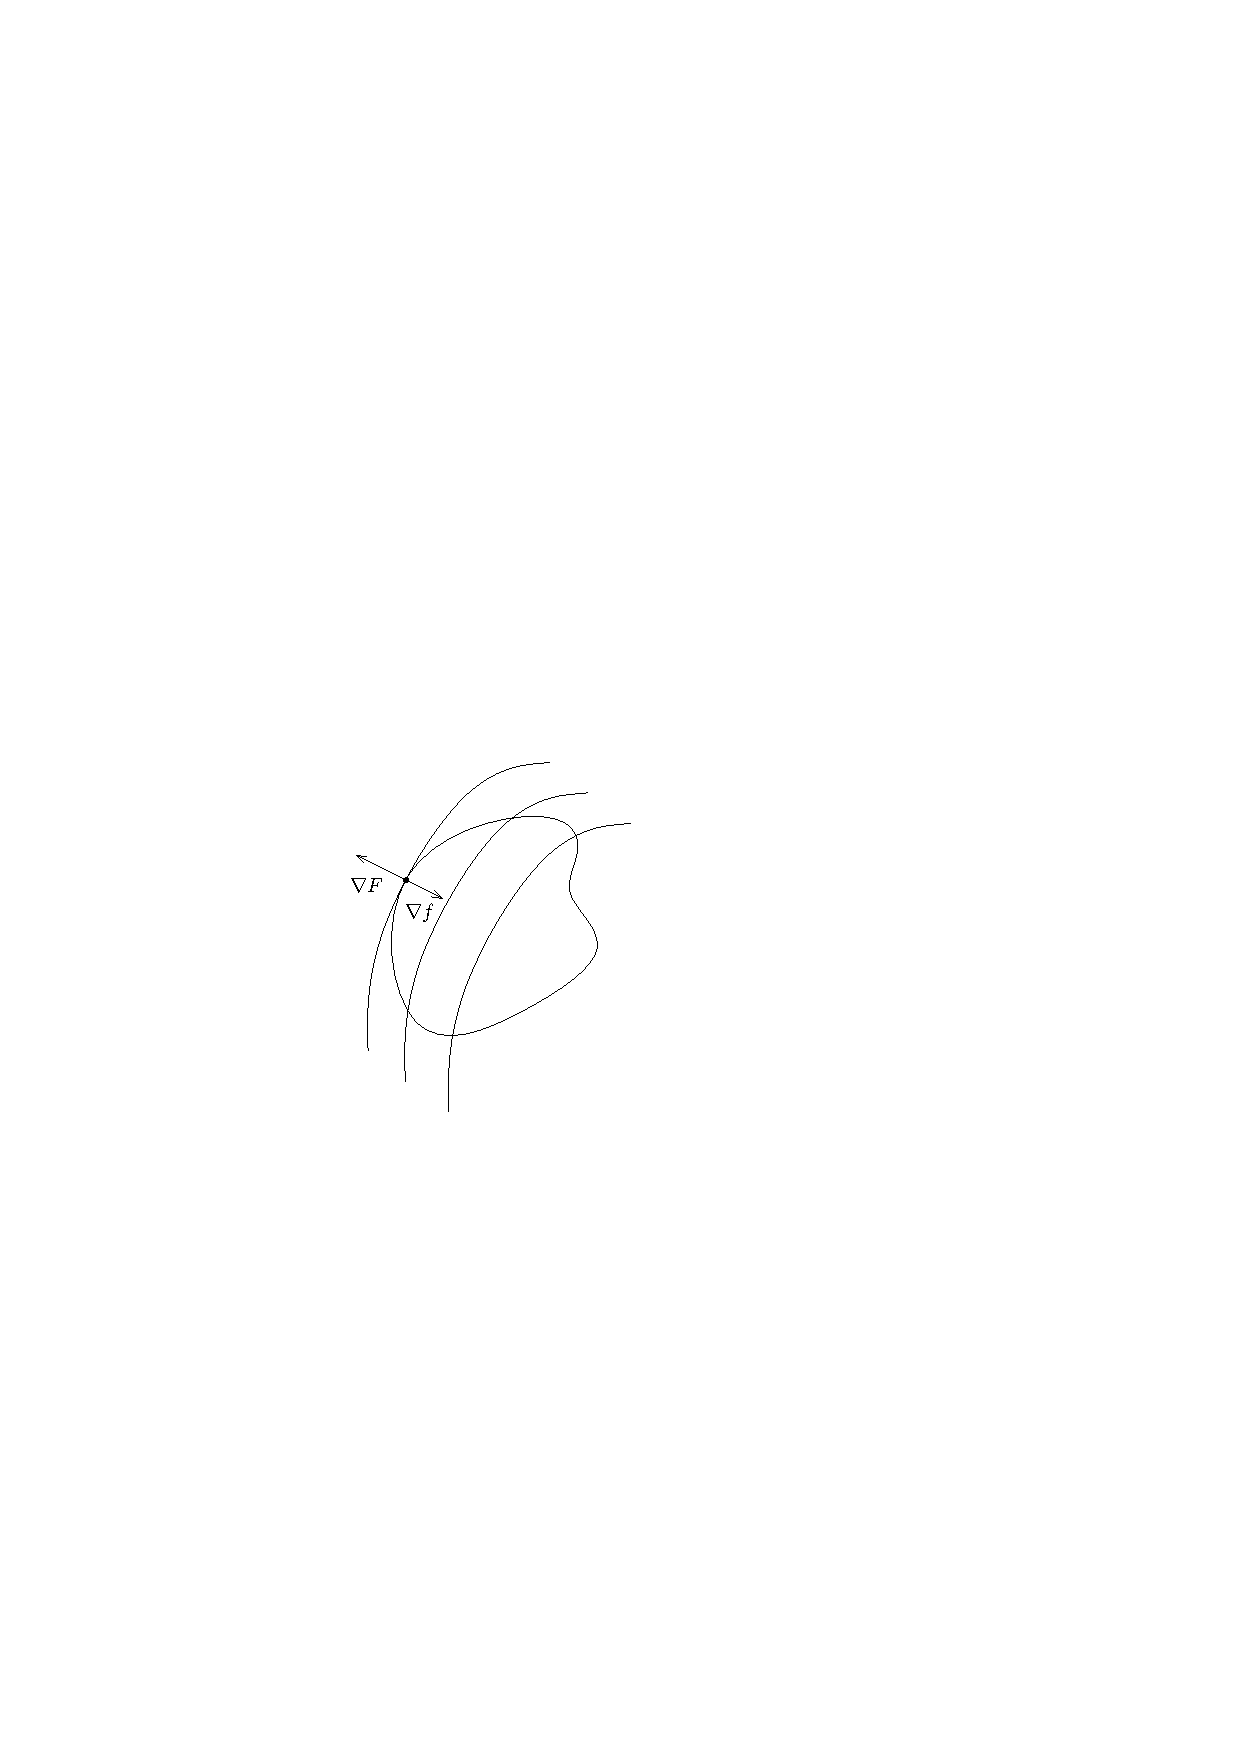
\includegraphics[width=0.6\textwidth]{condextr2d}
  \end{minipage} \hfill
  \begin{minipage}{0.48\linewidth}
    \[\nabla f = \lambda \nabla F\]
\begin{cor}[Правило Лагранжа]
  $f$ имеет в $a$ экстремум при условии $F_1(a) = \cdots = F_m(a) = 0$, то
  \begin{enumerate}
    \item либо $\nabla F_1(a), \dotsc, \nabla F_m(a)$ ЛЗ
    \item либо $\exists\, \lambda_1, \dotsc, \lambda_m \in \R \colon \nabla f(a) =
      \sum_i \lambda_i \nabla F_i(a)$ 
  \end{enumerate}
\end{cor}
  \end{minipage}
\end{exmp*}


\paragraph{Доказательство теоремы об условном экстремуме}
\label{par:diffspace::condextrema} 

\begin{ittproof}
  \begin{enumerate}
    \item Пусть $m = n - 1$. Будем доказывать от противного. Пусть в $a$ условный $\max$, но
      $\nabla f(a)$, $\nabla F_1(a), \dotsc, \nabla F_m(a)$~--- ЛНЗ.

      Рассмотрим $\Phi(x) = (f(x), F_1(x), \dotsc, F_m(x))$. Тогда такое $\Phi\colon G \to \R^n$.
      Из линейной независимости градиентов
      \[
        \Phi'(a) = \begin{pmatrix}
          \nabla f(a) \\ \nabla F_1(a) \\ \vdots \\ \nabla F_m(a) 
        \end{pmatrix}, \; \det \Phi'(a) \neq 0
      \]
      Пусть $b = \Phi(a) = (f(a), 0, \dotsc, 0)$. Тогда по теореме об обратном отображении 
      (\ref{thrm:diffspace::invsmooth}) 
      \[
        \exists\, U(a), V(b) \;\colon\; \Phi\colon U \to V \text{~--- диффеоморфизмъ}
      \]
      Пусть $V \supset B_\varepsilon(b)$, $y = (f(a)+ \frac{\varepsilon}{2}, 0, \dotsc, 0) \in V$, 
    тогда $\exists!\, x\in U \colon \Phi(x) = y$. Получается, что $f(x) > f(a)$, $\forall\, i\;
    F_i(x) = 0$, что немного противоречит тому, что в $a$ условный $\max$.
  \item Теперь рассмотрим случай $m < n - 1$ (всё остальное неинтересно, точно будет ЛЗ). \\
    Будем доказывать от противного. Пусть в $a$ условный $\max$, но
    $\nabla f(a)$, $\nabla F_1(a), \dotsc, \nabla F_m(a)$~--- ЛНЗ.
    Тогда $\rk \Phi'(a) = m+1 < n$. Добавим ещё функций $F_{m+1}, \dotsc, F_{n-1}$ таких, что
    $F_i(x) = x_{i+1} - a{i+1}$.

    Введём ещё стандартное обозначение
    \[
      x = (\underbrace{x, \dotsc, x_{m+1}}_{\bar{x}}, \underbrace{x_{m+2}, \dotsc,
      x_n}_{\bar{\bar{x}}})
    \]
    И не совсем стандартное
    \[
      A = \pder{(f_1, F_1, \dotsc, F_m)}{x_1, \dotsc, x_{m+1}}(a)
    \]
    Обычно такой <<дробью>> обозначают якобиан, но, пожалуй, сохраню обозначения с лекции.

    Итак
    \[
      \Phi'(a) = \left(
        \begin{array}{c|c}
          A & * \\
          \hline
          0 & E_{n-m-1}
        \end{array}
      \right) \Rightarrow \rk \Phi'(a) = n
    \]
    A теперь можно подвести всё к первому пункту.
    Рассмотрим $\widetilde{M} = \{x \mid F_1(x) = \cdots = F_{n-1}(x) = 0 \}$ (а 
    $M =  \{x \mid F_1(x) = \cdots = F_{m}(x) = 0 \}$). Поскольку $\widetilde{M} \subset M$,
    $f$ будет иметь в $a$ максимум и относительно $\widetilde{M}$.
    
    Аналогично 1 пункту получаем бред какой-то.
  \end{enumerate}
\end{ittproof}
\begin{rem}
  Такая теорема может найти лишь точки, <<подозрительные>> на экстремум. Надо ещё отдельно
  думать. Например, вдруг там на компакте всё определено.
\end{rem}
\begin{rem}
  Можно рассматривать функцию Лагранжа:
  \[
    \mathcal L (x) = f(x, \lambda) - \sum_{i=1}^m \lambda_i F_i(x)
  \]
  Тогда если в $a$ условный экстремум, то в $(a,\lambda_)$ стационарная точка 
  ($\mathcal L'(a) = 0$) функции Лагранжа.
  
\end{rem}





\end{document}
% vim: wrapmargin=3
